\documentclass[11pt]{article}
\usepackage[margin=0.8in]{geometry}
\usepackage[T1]{fontenc}
\usepackage{lmodern,amsmath,xcolor,listings,booktabs,array,longtable,enumitem,needspace}
\usepackage[titles]{tocloft}
\usepackage{tikz}
\usetikzlibrary{arrows.meta,positioning}
\usepackage[hidelinks,bookmarksopen=false]{hyperref}
\definecolor{ink}{RGB}{25,60,95}
\definecolor{codebg}{RGB}{247,248,250}
\setlength{\parindent}{0pt}
\setlength{\parskip}{5pt}
\setlength{\emergencystretch}{2em}
\setlist{nosep,leftmargin=1.4em,topsep=3pt}
\setcounter{tocdepth}{1}
\setlength{\cftbeforesecskip}{2pt}
\newcolumntype{L}[1]{>{\raggedright\arraybackslash}p{#1}}
\lstdefinestyle{base}{basicstyle=\ttfamily\small,keywordstyle=\color{ink}\bfseries,
commentstyle=\color{black!55},showstringspaces=false,columns=fullflexible,
keepspaces=true,breaklines=true,upquote=true,tabsize=4,frame=single,
rulecolor=\color{black!12},backgroundcolor=\color{codebg},aboveskip=5pt,belowskip=5pt}
\lstdefinestyle{sv}{style=base,language=Verilog,
morekeywords={logic,always_comb,always_ff,typedef,enum,localparam,int,signed,genvar}}
\lstdefinestyle{py}{style=base,language=Python,morekeywords={async,await}}
\lstnewenvironment{svcode}{\lstset{style=sv}}{}
\lstnewenvironment{pycode}{\lstset{style=py}}{}
\newcommand{\cd}[1]{{\frenchspacing\texttt{\detokenize{#1}}}}
\newcommand{\svfile}[1]{\par\noindent\begin{minipage}{\linewidth}\lstinputlisting[style=sv]{#1}\end{minipage}\par}
\newcommand{\svpart}[3]{\par\noindent\begin{minipage}{\linewidth}\lstinputlisting[style=sv,firstline=#2,lastline=#3]{#1}\end{minipage}\par}
\newcommand{\pyfile}[1]{\par\noindent\begin{minipage}{\linewidth}\lstinputlisting[style=py]{#1}\end{minipage}\par}
\newcommand{\transfer}[1]{\par\textbf{For a new design.} #1\par}
\newcommand{\sect}[1]{\hyperref[sec:#1]{\S\ref*{sec:#1}}}
\newcommand{\repo}[2]{\href{https://github.com/tiny-tpu-v2/tiny-tpu/blob/04ad69238072369ac3b5c43c495a3124b62a95aa/#1}{#2}}
\begin{document}
\begin{center}
{\LARGE\bfseries RTL and SystemVerilog Refresher}\\[5pt]
{\large Fundamentals, memory, datapaths, control, and verification}\\[4pt]
{\small Understand the hardware. Name the state. Trace the clock edge.}
\end{center}
This guide is for returning to RTL after time away. Start with the language and clocked-hardware model.
Then review the reusable blocks, memory interfaces, and design tradeoffs.
The tiny-tpu project supplies concrete connections; the examples teach general design rules.
The final sections give a small cocotb workflow and practice tasks for a 90-minute exercise.

For each topic, recover the purpose before the syntax. Explain why the update works, write the block, then change one assumption.
Runnable examples are in \cd{examples/}; their tests check cycle behavior and boundary cases.
\tableofcontents
\newpage

\section{Think in hardware and cycles}\label{sec:model}
The goal of RTL is to describe state and the logic that updates it.
Registers preserve bits across cycles. Combinational logic computes outputs from current inputs and register values.
Modules operate concurrently; source-file order does not schedule hardware modules.

\begin{center}
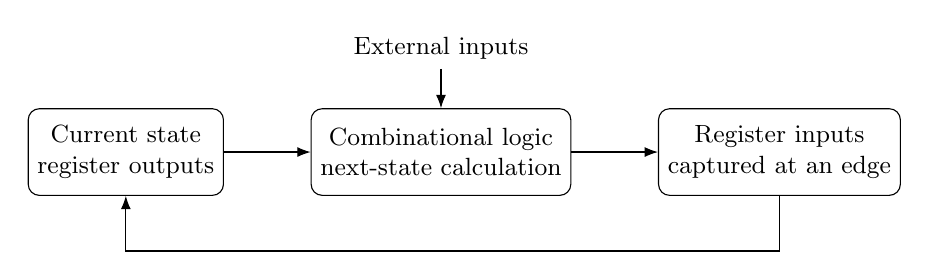
\begin{tikzpicture}[node distance=11mm,>=Latex,
every node/.style={font=\small},box/.style={draw,rounded corners,align=center,minimum height=11mm}]
\node[box] (q) {Current state\\register outputs};
\node[box,right=of q] (c) {Combinational logic\\next-state calculation};
\node[box,right=of c] (d) {Register inputs\\captured at an edge};
\draw[->] (q)--(c); \draw[->] (c)--(d);
\draw[->] (d.south)--++(0,-7mm)-|(q.south);
\node[above=5mm of c] (i) {External inputs}; \draw[->] (i)--(c);
\end{tikzpicture}
\end{center}
The feedback path passes through registers. A combinational feedback loop usually has no well-defined settling behavior for ordinary RTL design.

\textbf{Before coding, define the contract.}
\begin{enumerate}
\item What is transferred, and how wide is it? Is it signed? Is it an integer or fixed-point value?
\item Which edge accepts an input? What makes the input valid? Can either side stall?
\item What latency and sustained throughput are required? Can multiple operations be in flight?
\item What does reset clear? What happens on simultaneous operations or a boundary condition?
\end{enumerate}
For example: ``This block stores one byte. It accepts a byte when valid and ready are high at a rising edge.
It preserves that byte until the receiver accepts it. Reset discards any pending byte.''
That contract determines the register, valid bit, and enable equation in \sect{handshake}.

\textbf{Separate elaboration, synthesis, and simulation.}
Parameters and generate loops build a fixed circuit before simulation runs.
Synthesis maps supported RTL into gates, registers, and available memory resources.
Simulation also permits software-like testbench features such as delays and file access; those features do not automatically describe implementable hardware.
\transfer{Write one sentence for each stored fact and each externally visible timing rule.
If you cannot say which bits must survive to the next cycle, sketch the datapath before adding an FSM.}

\section{The SystemVerilog syntax you need}\label{sec:syntax}
\subsection{Modules, ports, signals, and connections}
A module is a hardware boundary. Ports connect it to other hardware.
Declare vector widths explicitly and use named connections so that port order cannot silently change the wiring.
\par\noindent\begin{minipage}{\linewidth}
\begin{svcode}
logic [7:0] a, b;
logic [8:0] sum;
assign sum = {1'b0, a} + {1'b0, b};

counter #(.LIMIT(10)) u_counter (
    .clk(clk), .rst(rst), .en(en), .count(count), .tick(tick)
);
\end{svcode}
\end{minipage}\par
\cd{logic} is a four-state variable type, not an instruction to build a flip-flop.
Its assignment context determines whether it represents combinational logic or registered state.
\cd{wire} is a net type used for connections and continuous drivers. Legacy \cd{reg} denotes a procedural variable; it does not necessarily mean a hardware register either.
For ordinary internal signals, give each signal one owner. Do not assign one register from two procedural blocks.

\begin{longtable}{@{}L{5.6cm}L{10.4cm}@{}}
\toprule Syntax & Meaning and example \\ \midrule\endhead
\cd{logic [7:0] data} & One 8-bit packed vector. \cd{data[0]} is its least significant bit.\\
\cd{logic signed [7:0] delta} & Signed two's-complement value: range \(-128\) through 127. Packed vectors are unsigned unless declared signed.\\
\cd{logic [7:0] mem [0:15]} & An unpacked array of sixteen 8-bit words. \cd{mem[3][0]} selects one word's low bit.\\
\cd{logic [1:0][7:0] lanes} & One packed object containing two 8-bit lanes; it can also be treated as a 16-bit vector.\\
\cd{parameter int W = 8} & Configurable elaboration constant. \cd{localparam} is derived locally and cannot be overridden.\\
\cd{typedef enum logic [1:0]} & Name a state type and its encodings; use named states instead of unexplained bit patterns.\\
\cd{typedef struct packed} & Group named fields into one packed vector, useful for an instruction or a data/metadata bundle.\\
\bottomrule
\end{longtable}

\subsection{Literals, slicing, concatenation, and operators}
Use sized constants to make bit patterns visible. For example, \cd{8'hFF} is eight one-bits; \cd{8'shFF} is the signed value \(-1\).
An unsized decimal literal such as \cd{1} introduces integer sizing and signedness rules. Prefer explicit widths at RTL boundaries.
\par\noindent\begin{minipage}{\linewidth}
\begin{svcode}
logic [15:0] word;
logic [7:0] byte_value;
assign byte_value = word[15:8];      // constant part select
// word[base +: 8] selects 8 bits starting at base and going up.
// word[base -: 8] selects 8 bits starting at base and going down.
// The base may vary; the selected width must be constant.
assign word = {8'hA5, 8'h3C};        // concatenation: 16'hA53C
// {4{2'b10}} is replication: 8'b10101010.
// '0 fills the destination width with zeros; '1 fills it with ones.
\end{svcode}
\end{minipage}\par
This is a syntax fragment: the output slice follows the continuously driven word, which is a constant in this example.
Concatenation joins bit fields; replication repeats a pattern.

\begin{longtable}{@{}L{5.6cm}L{10.4cm}@{}}
\toprule Operator & What to recall \\ \midrule\endhead
\cd{+ - * /} & Arithmetic. Constant power-of-two operations can simplify; general division can be expensive hardware.\\
\cd{& | ^ ~} & Bitwise AND, OR, XOR, NOT. \cd{4'b1010 & 4'b1100} gives \cd{4'b1000}.\\
\cd{&& || !} & Logical tests. \cd{4'b0010 && 4'b0100} is true even though their bitwise AND is zero.\\
\cd{&data}, \cd{|data}, \cd{^data} & Reduce all bits to one bit: all-set, any-set, or parity.\\
\cd{== !=}, \cd{< <= > >=} & Value comparisons. Signedness of the expression matters. In an expression, \cd{<=} means less-than-or-equal.\\
\cd{=== !==} & Simulation case equality: X and Z are compared as symbols. Useful in tests, not a substitute for an RTL unknown-value policy.\\
\cd{<< >> >>>} & Left shift, zero-fill right shift, and arithmetic right shift. \cd{>>>} sign-extends only when its left operand is signed.\\
\cd{condition ? a : b} & A mux. Keep branch widths and signedness consistent.\\
\bottomrule
\end{longtable}
\cd{X} means unknown in four-state simulation; \cd{Z} means high impedance.
An unknown comparison can produce X; an \cd{if} does not treat X as definitely true.
Avoid \cd{casex} for normal control logic because it can hide real unknowns.

\subsection{Widths and signedness are part of the arithmetic}
The goal is to preserve the intended numeric range, not just to silence a warning.
Two 8-bit unsigned inputs can sum to 510, so the full sum needs 9 bits.
Widen operands explicitly when the intermediate result must be preserved.
\par\noindent\begin{minipage}{\linewidth}
\begin{svcode}
logic [7:0] a, b;
logic [8:0] full_sum;
assign full_sum = {1'b0, a} + {1'b0, b};
// a=200, b=100: full_sum=300; truncating to 8 bits gives 44.

logic signed [7:0] x, y;
logic signed [8:0] signed_sum;
assign signed_sum = $signed({x[7], x}) + $signed({y[7], y});
// x=-100, y=-100: signed_sum=-200.
\end{svcode}
\end{minipage}\par
SystemVerilog uses context-dependent expression widths; the destination can affect some arithmetic expressions.
Do not assume that every operation has either unlimited width or always the operand width.
Explicit extension makes the intended intermediate width visible.
\cd{$signed(value)} changes interpretation, not the bit count or binary-point position.
A part select and a concatenation are unsigned unless cast or assigned into a suitable signed context.
For example, casting \cd{8'hFF} to signed gives \(-1\); zero-extending it to \cd{16'h00FF} gives 255.

\subsection{Loops build repeated work or repeated hardware}
A combinational loop with a fixed bound describes repeated logic, not several clock cycles.
A loop inside a clocked block still executes for one clock event.
Use a counter and state when work must be spread across cycles.
\svfile{examples/lane_adders.sv}
The generate loop creates \cd{LANES} adders. \cd{genvar} is an elaboration index.
For a small helper calculation, a synthesizable \cd{function automatic} can express combinational logic without copied code.
A function does not insert a cycle or create a background software task.

\textbf{Parameter edge cases.} An address for \cd{DEPTH} entries needs \cd{$clog2(DEPTH)} bits, but \cd{$clog2(1)} is zero.
Guard it with a minimum width of one. A count from 0 through \cd{DEPTH} needs \cd{$clog2(DEPTH+1)} bits.
These are different ranges.
\transfer{Before choosing a cast or slice, state the source range, required intermediate range, and destination range.
Before writing a loop, decide whether the goal is parallel hardware or one operation reused across cycles.}

\section{Combinational logic and clocked state}\label{sec:state}
\subsection{Combinational logic must decide every output}
Use blocking assignments in \cd{always_comb}. Set defaults, then override them.
An unassigned output must retain its previous value, which can infer a latch.
\par\noindent\begin{minipage}{\linewidth}
\begin{svcode}
always_comb begin
    result = '0;
    valid = 1'b0;
    if (enable) begin
        result = a + b;
        valid = 1'b1;
    end
end
\end{svcode}
\end{minipage}\par
The hardware is a mux and an adder. Assigning zero on the disabled path is a deliberate behavior.
If the requirement is to preserve the previous value, express an enabled register in \cd{always_ff} instead.
For a state decoder, use a default next state and a normal \cd{case} with a defined fallback.
\cd{unique case} expresses a checking/optimization intent; it does not replace complete assignments or correct encodings.

\subsection{At an edge, every register reads the old state}
Use nonblocking assignments for register updates. Right-hand sides are evaluated using the state visible when the block executes;
the scheduled updates become visible later in that simulation time step.
\par\noindent\begin{minipage}{\linewidth}
\begin{svcode}
always_ff @(posedge clk) begin
    a <= b;
    b <= a;
end
\end{svcode}
\end{minipage}\par
If the old values were \cd{a=1, b=2}, the new values are \cd{a=2, b=1}.
This describes two registers exchanging values. It does not perform a sequential software copy.
With \cd{a = b; b = a;} in one procedural execution, the second statement would read the changed \cd{a}.

\par\noindent\begin{minipage}{\linewidth}
\begin{svcode}
always_ff @(posedge clk) begin
    if (rst) q <= '0;
    else if (en) q <= d;
end
\end{svcode}
\end{minipage}\par
There is no assignment when \cd{en} is false, so the flip-flop holds its value. That is intentional state retention, not a latch.
Omitting a register from reset can also be intentional if a reset valid bit makes its data irrelevant.
Within one block, later executed nonblocking assignments to the same variable override earlier ones for that edge.
Prefer one clear priority chain; never depend on scheduling order between separate blocks.

\subsection{A counter makes the boundary explicit}
The counter runs from zero to \cd{LIMIT-1}. An enabled terminal edge wraps it and produces one cycle of \cd{tick}.
Reset has priority over enable.
\svfile{examples/counter.sv}
\cd{CW'(LIMIT-1)} is a sized cast to \cd{CW} bits.
For \cd{LIMIT=3} and enable continuously high, post-edge counts are \cd{1,2,0,1,2,0}; ticks are \cd{0,0,1,0,0,1}.
For \cd{LIMIT=1}, every enabled edge is terminal. The guarded width keeps that configuration legal.
\transfer{Write a table of old state, input conditions, and new state.
Resolve priority explicitly when reset, load, clear, and increment can coincide.}

\section{FSMs: control the progress of one transaction}\label{sec:fsm}
An FSM is useful when the same datapath does different work on different cycles.
The state should describe the transaction's progress, not merely label lines of code.

Consider a block that sums exactly \cd{N} incoming bytes. A start command captures \cd{N}; input bubbles must not consume a byte.
Use three states: IDLE accepts a command, RUN accepts data, DONE reports completion for one cycle.
\begin{longtable}{@{}L{3cm}L{6cm}L{7cm}@{}}
\toprule State & Event & Action / next state \\ \midrule\endhead
IDLE & Start with \(N>0\) & Clear sum, capture count, enter RUN.\\
IDLE & Start with \(N=0\) & Clear sum and enter DONE.\\
RUN & Valid input accepted & Add data and decrement remaining count; enter DONE on the last accepted item.\\
RUN & No accepted input & Hold sum and remaining count.\\
DONE & Next edge & Return to IDLE.\\
\bottomrule
\end{longtable}
The remaining count means ``items still to be accepted'', so its old value is 1 on the final transfer.
Do not decrement merely because a cycle passed.
\svpart{examples/stream_sum.sv}{11}{29}
The next-state block computes only a decision. The sequential block owns the stored state and datapath registers.
\svpart{examples/stream_sum.sv}{30}{45}
The full file supplies the ports and declarations. \cd{in_ready} is true only in RUN; \cd{done} is true in DONE.
The final data edge updates both \cd{sum} and the state, so the completed sum is available while \cd{done} is high.
Starts while busy are ignored by this contract. A held start can launch another command once IDLE returns; use a pulse or a proper command handshake.
\transfer{Separate command acceptance, request issue, response wait, and completion when their events occur on different cycles.
Capture command fields once instead of letting a busy transaction follow live input wires.}

\section{Ready/valid: preserve work under backpressure}\label{sec:handshake}
The goal is to let either side pause without losing, duplicating, or changing an item.
Outside reset, a transfer occurs at a rising edge when \cd{valid && ready} is true.
The sender owns valid and data; the receiver owns ready.
Once valid is asserted, the sender keeps valid and the same data until acceptance.
It must not wait for ready before making a pending item valid.

\subsection{Derive a one-entry elastic register}
Store the data and a bit saying whether the slot is occupied.
The slot can accept input if it is empty or if the receiver will remove the current item at this edge.
Therefore \cd{in_ready = !out_valid || out_ready}.
\svfile{examples/rv_register.sv}
When stalled with a valid output, \cd{in_ready} is false and the block changes nothing.
When an old item leaves, a new item can replace it at the same edge.
When no new item arrives and the old one leaves, the valid bit clears.
The data register is not reset because its value is meaningful only when valid is high.

\begin{longtable}{@{}L{4.8cm}L{11.2cm}@{}}
\toprule Pre-edge condition & Result after the edge \\ \midrule\endhead
Empty, new valid item A & A occupies the slot. It was not also transferred to the receiver through an empty bypass.\\
Occupied by A, receiver stalled & A and output valid hold. No input is accepted.\\
Occupied by A, receiver ready, new B valid & A transfers out; B replaces it. Occupancy stays one.\\
Occupied by A, receiver ready, no new input & A transfers out; the slot becomes empty.\\
\bottomrule
\end{longtable}
This block can sustain one item per cycle after filling. It adds a register boundary, not an empty-path combinational bypass.
Several such stages can form a long combinational ready path. Registering ready alone is unsafe if an already accepted item then has nowhere to go.
Break that path with a correctly sized skid/elastic buffer, or use credits that reserve storage.
\transfer{Define transfers from pre-edge values. Attach all metadata to the same acceptance and stall rules as its data.
Before adding a register to a control path, account for every item that may still arrive before the sender observes the stall.}


\section{FIFO: derive the state from occupancy}\label{sec:fifo}
A FIFO absorbs a temporary difference between production and consumption rates while preserving order.
Store the words, a read pointer, a write pointer, and the number of occupied slots.
Define \cd{push} and \cd{pop} from accepted transfers, not from requests alone.
\begin{longtable}{@{}L{3cm}L{3cm}L{10cm}@{}}
\toprule Push & Pop & Occupancy change \\ \midrule\endhead
0 & 0 & Hold.\\
1 & 0 & Add one.\\
0 & 1 & Subtract one.\\
1 & 1 & Hold; both pointers advance.\\
\bottomrule
\end{longtable}
The invariant is \(0\leq\text{count}\leq\text{DEPTH}\).
Empty means count is zero; full means count equals depth.
A full FIFO can accept a replacement when the old head will leave at the same edge.
An empty FIFO cannot pop in this design, even if a new input arrives at that edge.
\svfile{examples/sync_fifo.sv}
The casts \cd{AW'(...)} and \cd{CW'(...)} size constant comparisons explicitly.
The pointer width represents addresses; the count width must also represent DEPTH itself.
Explicitly wrapping at \cd{DEPTH-1} supports depth 3 as well as powers of two.
At depth 1, simultaneous push/pop transfers the old word and replaces it with the new word.
Reset discards all entries by clearing pointers and count; it need not clear the data array.

The head read is combinational. This is useful for a small register-based FIFO, but it does not match a synchronous-read SRAM directly.
With synchronous SRAM, request the head in advance and hold the returned word in an output register.
Track both stored words and any outstanding read so that prefetch does not duplicate or skip a word.
\transfer{Choose the memory interface before choosing FIFO control. Ask whether an input may bypass an empty FIFO,
whether a full FIFO may accept during a pop, and whether ready can depend combinationally on downstream ready. Those choices determine the boundary logic.}

\section{Memory: separate the interface from the storage}\label{sec:memory}
\subsection{Registers, SRAM, and DRAM}
An RTL array describes indexed storage. It does not, by itself, promise a physical memory macro.
The access pattern, reset behavior, synthesis tool, and target technology determine the implementation.
\begin{longtable}{@{}L{2.3cm}L{6.7cm}L{7cm}@{}}
\toprule Storage & Useful mental model & Design consequence \\ \midrule\endhead
Registers & Individually accessible state bits with surrounding mux logic. & Flexible ports and reset, but large arrays and wide selection muxes cost area and timing.\\
SRAM & Dense static storage with a fixed set of ports and a defined timing contract. & Match port count, access latency, masks, and collision behavior. An ASIC macro is an explicit implementation resource.\\
DRAM & Dense dynamic storage, usually reached through a controller and PHY. & Refresh, row operations, scheduling, and bursts affect service time. Buffer requests and responses.\\
\bottomrule
\end{longtable}
A \textbf{1RW} memory has one port that reads or writes. A \textbf{1R1W} memory has a read port and a write port.
A \textbf{2RW} memory has two read/write ports, with specified restrictions on collisions.
``Dual port'' alone does not define which operations may occur together.
Two addresses in one cycle require two available accesses, separate banks, replication, or a schedule that serializes them.

\subsection{A synchronous-read RAM model}
The request address and enable are sampled at a rising edge. Read data and its valid bit update after that edge.
The model below accepts one read and one write per cycle, with valid addresses in \cd{0..DEPTH-1}.
It specifies old data when the same address is read and written at the same edge.
\svfile{examples/sync_ram.sv}
Both right-hand sides see the pre-edge memory contents. A later write statement does not make this a new-data read.
A physical macro may instead return new data, preserve its old output, or leave that collision undefined.
Match the macro's specification, or add forwarding/arbitration to provide the external behavior you need.

\begin{longtable}{@{}L{3cm}L{6.5cm}L{6.5cm}@{}}
\toprule Time & RAM & A separate downstream register \\ \midrule\endhead
Before edge E0 & Read enable and address A are stable. & Sees the previous response.\\
At E0 & Samples the request. & Still samples the previous response, not A's new data.\\
After E0 settles & \cd{rd_valid=1}; \cd{rd_data=mem[A]}. & Combinational consumers can now use A's response.\\
At E1 & May accept the next request. & Can capture A's response.\\
\bottomrule
\end{longtable}
Calling this a one-cycle read is common, but an edge table removes ambiguity.
A controller that issues a request and consumes its response in the same sequential step will use stale data.

\subsection{Reset, ports, addresses, and inference}
Reset valid bits and ownership state first. A large loop that clears every word in one clock asks for hardware that writes every word at once;
an ordinary SRAM cannot do that. If contents must be initialized, use an initialization sequence, valid tags, or a supported memory initialization mechanism.
Unwritten locations in this model are unspecified; do not test them as zero.

A byte address and a word index are different. In a byte-addressed system with aligned 32-bit words,
address 12 selects word index 3; the two low address bits select a byte within the word.
Four byte enables permit partial writes without replacing the other bytes, if the memory supports them.
For a 16-bit word, two byte lanes are enough. Check alignment and the interface contract before shifting an address.

For FPGA RAM inference, use the vendor's supported template and confirm the synthesis report.
For an ASIC, a macro wrapper must match the macro's functional model, timing view, physical view, and pin polarities.
A declaration with three independent reads does not become a two-port SRAM merely because it is called a buffer.
\transfer{List every access that must occur in one cycle. Then assign each access to a real port or bank.
Treat latency, read/write collisions, byte masks, and reset as interface requirements, not implementation details to discover later.}

\section{DRAM: enough architecture to reason about a controller}\label{sec:dram}
DRAM stores charge that must be refreshed. Think of a bank as having rows and a currently open row.
An ACTIVATE opens a row; READ or WRITE commands move column data in bursts; PRECHARGE prepares the bank to open another row.
These commands have timing constraints. A row hit can avoid closing and reopening a row, but it still obeys column and bus timing.

\begin{longtable}{@{}L{3cm}L{13cm}@{}}
\toprule Term & What it constrains \\ \midrule\endhead
\(t_{\mathrm{RCD}}\) & Delay from ACTIVATE to a permitted READ/WRITE.\\
\(t_{\mathrm{RP}}\) & Time after PRECHARGE before a subsequent ACTIVATE.\\
\(t_{\mathrm{RAS}}\) & Minimum time a row stays active before it can be precharged.\\
\(t_{\mathrm{RFC}}\) & Refresh recovery time, according to the device's refresh mode.\\
\bottomrule
\end{longtable}
For example, a conflicting row request may require PRECHARGE, a wait, ACTIVATE, another wait, then a column command and data transfer.
Other constraints also apply: command spacing, write recovery, read/write turnaround, and interactions across banks.
Use the selected device/controller specification for actual values; these four names are not a complete scheduler.
An RTL client normally talks to a controller's request/response interface rather than driving DRAM pins directly.

\textbf{Latency and bandwidth solve different problems.}
Latency is how long one request takes. Bandwidth is how much data can be sustained over time.
If a downstream interface can return 16 bytes per cycle but a request takes 20 cycles to return,
roughly \(16\times20=320\) bytes of useful work must be in flight to cover that delay at full rate.
That is twenty 16-byte responses, assuming enough independent requests and no other bottleneck.
One outstanding request followed by a wait cannot achieve that throughput.

Use bursts for contiguous tiles, buffer responses, and reserve destination capacity before issuing work that cannot be stopped.
Track accepted requests separately from received responses. A burst counter advances on accepted beats, not merely on elapsed clocks.
If response order is not guaranteed, carry transaction IDs and reorder or route results correctly.
\transfer{Ask what limits useful throughput: request issue rate, outstanding capacity, row/bank conflicts, data-bus use, or consumption rate.
Buffering can hide latency; it cannot create memory bandwidth.}

\section{Arithmetic, MACs, and fixed-point values}\label{sec:arithmetic}
\subsection{Choose the numeric range before the width}
Multiplying two signed W-bit integers requires up to 2W bits for the full product.
Adding up to K such products needs a conservative extra \(\lceil\log_2 K\rceil\) bits, assuming no larger initial bias or accumulator value.
For sixteen signed 8-bit products, a 20-bit accumulator is a safe choice: \(16+4=20\).
The width is a range budget, not a rule that makes arbitrary later additions safe.
\svfile{examples/mac.sv}
This block computes one signed integer MAC result at an accepting edge and registers its valid flag with that result.
It has no ready input; it accepts every valid cycle and cannot absorb downstream backpressure.
The separate signed \cd{product_extended} makes sign extension into the accumulator width explicit.
Overflow wraps here. Saturation would require computing a wider result and clamping it before narrowing.

\subsection{A binary point is an interpretation of stored bits}
For a signed 16-bit value with 8 fractional bits, the real value is stored integer divided by 256.
Its range is \(-128\) through \(127+255/256\).
This guide uses ``16 bits, F=8'' to avoid differing conventions for whether Q-format integer bits include the sign.

For example, 1.5 is stored as 384, and \(-0.5\) is stored as \(-128\).
Their full product is \(-49152\), now with 16 fractional bits.
To return to F=8, shift the wide signed product right by 8: \(-192\), representing \(-0.75\).
\par\noindent\begin{minipage}{\linewidth}
\begin{svcode}
logic signed [15:0] a, b;
logic signed [31:0] product, scaled;
assign product = a * b;        // F=16 when inputs have F=8
assign scaled = product >>> 8; // F=8, still wide
// Check scaled against the 16-bit limits before narrowing.
\end{svcode}
\end{minipage}\par
Arithmetic right shift rounds negative nonmultiples toward negative infinity: \(-3\mathbin{>>>}1=-2\).
It is not truncation toward zero. State whether you want floor, nearest with a defined tie rule, or another policy.
Do not add a universal ``rounding constant'' without checking negative values and tie handling.

Addition requires the same binary-point position. For example, align a bias to the accumulator's scale before adding it.
Keeping full products through a dot product and rounding once usually loses less precision than rounding each product,
but it costs wider storage and adders. Repeated per-PE requantization can produce a different numerical answer.
A sticky overflow bit records that an error occurred; it does not repair the result.
\transfer{Write the signed range and fractional-bit count on every arithmetic boundary.
Then trace one positive value, one negative value, and one overflow case through extension, multiplication, rescaling, rounding, and narrowing.}

\section{Pipelines: move meaning with the data}\label{sec:pipeline}
A pipeline divides a long combinational calculation with registers.
\textbf{Latency} is the number of cycle intervals from acceptance to an available result.
\textbf{Initiation interval} is the spacing between accepted operations. A three-stage pipeline can have latency three and accept a new item every cycle.
Use an edge table to specify whether you count the input-capture edge as stage one.

Suppose stage 1 registers a product and stage 2 adds a bias. Stage 2 reads the previous product, so it must also read the previous item's bias and valid bit.
\par\noindent\begin{minipage}{\linewidth}
\begin{svcode}
// product1 is signed and wide enough; bias1/result use accumulator width.
always_ff @(posedge clk) begin
    if (rst) begin
        valid1 <= 1'b0;
        valid2 <= 1'b0;
    end else begin
        valid1 <= in_valid;
        valid2 <= valid1;
        if (in_valid) begin
            product1 <= x * weight;
            bias1 <= bias;
        end
        if (valid1)
            result <= product1 + bias1;
    end
end
\end{svcode}
\end{minipage}\par
At E0, item A enters stage 1. At E1, A's result enters stage 2 while B may enter stage 1.
After E1, \cd{valid2} describes A's result. A bubble at the input must produce a bubble at the corresponding output slot.
Tags, addresses, destination IDs, last-item flags, and operation modes need the same alignment as their data.

The example has no stalls. If a stage stalls, its data, valid, and metadata must all hold.
Either stall the whole pipeline under one enable, or give each stage its own elastic acceptance rule.
A freely running valid shift register beside a stalled datapath breaks alignment.
Changing an output mux mode while an older item is in flight can send that item down the wrong path; carry the mode or drain before changing it.

A pipelined multiplier in a feedback accumulator needs extra thought: the accumulator depends on an earlier result.
Track which partial sum belongs to each product, interleave independent accumulations, or accept a larger initiation interval.
Adding registers changes the schedule; it does not automatically preserve a recurrence.

\subsection{Double buffering and a weight commit edge}
Keep an active bank for computation and a shadow bank for loading the next job.
Ownership prevents the loader from changing values in use. Swap ownership only at a defined boundary.
\svfile{examples/weight_bank.sv}
With only \cd{active <= shadow}, a separate MAC sampling \cd{active} at the swap edge still uses the old active value.
The optional combinational \cd{selected} mux lets that MAC sample the pre-edge shadow value at the swap edge instead.
If load and swap are both asserted, active receives the old shadow while shadow receives the new input.
The mux does not magically forward that incoming load; that would require another explicit rule.
\transfer{Whenever a register is added, removed, enabled, or bypassed, trace data and its control through two consecutive items and one bubble.
For bank swaps, specify exactly which version a computation at the boundary must observe.}

\section{Timing, reset, and clock-domain boundaries}\label{sec:timing}
\subsection{What a timing path means}
For two registers on the same clock, a simplified setup condition is
\[
 t_{\mathrm{clk\to Q}}+t_{\mathrm{comb,max}}+t_{\mathrm{setup}}\leq T_{\mathrm{clk}}.
\]
Clock skew, uncertainty, and constraints modify the available budget.
A deep adder/mux chain can miss setup even when its functional simulation is correct.
Reduce logic depth, reduce fanout, change the arithmetic structure, or insert a pipeline register and update the protocol latency.

Hold checks concern the \emph{minimum} path delay just after the capturing edge.
Lowering the clock frequency generally does not fix a hold violation on a same-edge path.
Physical implementation tools add delay or change routing as needed under correct constraints.
RTL simulation verifies behavior; synthesis and static timing analysis answer different questions.

Use \cd{if (enable)} inside a clocked block for an enable.
Do not casually create a clock with \cd{clk & enable}: enable changes can make glitches or unintended edges.
ASIC clock gating uses dedicated glitch-safe cells and clock-tree/verification support; FPGA targets provide their own supported clock resources.

\subsection{Reset establishes a valid starting protocol state}
A synchronous reset takes effect only at the active clock edge. An asynchronous reset can assert without that edge.
Asynchronous reset release near an edge can violate recovery/removal timing; synchronize release within each clock domain when using that strategy.
Choose reset polarity and style to match the system and library rather than applying one style universally.
Reset FSMs, valid bits, pointers, and ownership as needed. Data bits may remain unreset when their validity makes them unobservable.
A synchronous reset cannot clear a block whose clock is stopped until that clock runs.

\subsection{Crossing a clock boundary changes the problem}
A receiving flip-flop can become metastable when an asynchronous signal changes near its sampling edge.
Two receiving-domain synchronizer registers reduce the chance that metastability propagates; they do not make the first register immune.
\par\noindent\begin{minipage}{\linewidth}
\begin{svcode}
// For a suitably stable single-bit level; reset style omitted here.
always_ff @(posedge dst_clk) begin
    sync1 <= async_level;
    sync2 <= sync1;
end
\end{svcode}
\end{minipage}\par
This does not guarantee capture of a narrow pulse. Use a pulse-stretch rule, a toggle protocol with a safe event spacing,
or a request/acknowledge handshake when every event must arrive.
Independently synchronizing the bits of a bus can capture a mixture of two words.
For occasional words, hold the bus stable under a handshake. For a stream, use a correctly designed asynchronous FIFO.

An asynchronous FIFO commonly crosses Gray-coded pointers through synchronizers, then derives local full/empty decisions.
Gray coding changes one bit per pointer step; it does not remove the need for the proper FIFO equations, synchronizers, physical CDC constraints, and reset protocol.
A ready/valid connection alone is not a clock-domain crossing solution.
\transfer{First identify whether two endpoints share a clock. Then choose a transfer protocol that preserves a level, event, word, or stream as required.
Do not start with ``add two flops'' before deciding what must be preserved.}

\section{Architecture: reuse, locality, and configurable datapaths}\label{sec:architecture}
\subsection{From a MAC to a systolic array}
For \(C_{ij}=\sum_k A_{ik}B_{kj}\), each output needs repeated multiply-add work.
A weight-stationary array keeps a weight in each PE. Activations move horizontally; partial sums move vertically.
Registers make each hop local and give a regular schedule.

In a two-row column, the upper PE can form \(a_0w_0+p\) at E0.
The lower PE can add \(a_1w_1\) to that partial sum at E1.
Therefore the matching lower-row activation must be present for E1, not merely arrive at the array at the same time as \(a_0\).
Likewise, an activation reaches a later column later. Boundary skew or equivalent internal delay aligns operands for each output.
An enable signal cannot correct a value that belongs to the wrong dot product.

\begin{center}
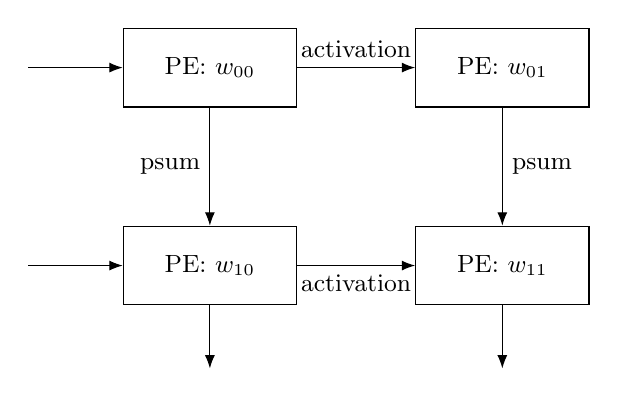
\begin{tikzpicture}[>=Latex,node distance=15mm,
every node/.style={font=\small},pe/.style={draw,minimum width=22mm,minimum height=10mm}]
\node[pe] (a) {PE: \(w_{00}\)};
\node[pe,right=of a] (b) {PE: \(w_{01}\)};
\node[pe,below=of a] (c) {PE: \(w_{10}\)};
\node[pe,right=of c] (d) {PE: \(w_{11}\)};
\draw[->] (a)--node[above]{activation}(b);
\draw[->] (c)--node[below]{activation}(d);
\draw[->] (a)--node[left]{psum}(c);
\draw[->] (b)--node[right]{psum}(d);
\draw[->] ([xshift=-12mm]a.west)--(a.west);
\draw[->] ([xshift=-12mm]c.west)--(c.west);
\draw[->] (c.south)--++(0,-8mm);\draw[->] (d.south)--++(0,-8mm);
\end{tikzpicture}
\end{center}
A fully occupied \(N\times N\) array can perform \(N^2\) MACs per cycle, if each PE supports one MAC per cycle and data arrives correctly.
That is peak arithmetic capacity. Small tiles, fill/drain cycles, missing operands, and memory stalls reduce useful utilization.
Count operations and transfers for a complete tile rather than quoting the peak alone.

\subsection{Choose reuse before increasing parallelism}
A scalar engine reuses one MAC over many cycles. Unrolling work creates more MACs and raises operand bandwidth demand.
Tiling keeps a useful subset of weights, activations, or partial sums near computation so that external memory traffic is amortized.
Choose the resident quantity from the access pattern: reuse weights across examples, activations across outputs, or keep partial sums local to avoid repeated writes.

Banking creates independent accesses when addresses land in different banks.
For B banks with simple word interleaving, \(\text{bank}=\text{word address}\bmod B\).
With four banks, addresses 0,1,2,3 can be read together from four single-read banks; addresses 0,4,8,12 conflict in bank 0.
Changing the layout or schedule can resolve the conflict. More compute lanes alone cannot.

Ping-pong tile buffers can overlap loading tile \(n+1\) with computing tile \(n\).
Ideal steady-state tile time approaches the larger of load time and compute time instead of their sum,
provided the memories, ports, and transfer engines actually permit overlap. Add startup/drain costs and any shared writeback bottleneck.

\subsection{A general view of a CGRA}
A coarse-grained reconfigurable array connects word-level processing elements with configurable operations and routes.
Compared with a fixed systolic path, it can map several datapaths by changing PE functions, routing, and schedules.
The design still obeys the same constraints: operand availability, port conflicts, route capacity, register boundaries, and numeric widths.

For example, mapping \((a+b)\times c\) requires an adder PE, a multiplier PE, and delivery of the matching \(c\).
If the adder result crosses one register boundary, delay \(c\) by the same amount or schedule its arrival later.
If two operands need the same single-port source memory at once, add a bank or change the schedule.
Keep routing configuration stable for in-flight work, carry configuration identity, or drain before reconfiguration.
Local neighbor routes are simple but constrain mappings; a broad crossbar is flexible but can cost area, wiring, and timing.
\transfer{For any accelerator, trace one output backward: which operands, stored where, arriving on which cycle, through which ports?
Then estimate useful operations per byte and ask whether the memory system can feed the chosen parallelism.}

\section{Cocotb: drive, predict, and check}\label{sec:cocotb}
Cocotb lets Python drive and observe an HDL simulation. The RTL still supplies clocked hardware behavior.
Start with one clock, a few inputs, an independent reference model, and assertions.
You do not need a large verification framework to test a counter, FIFO, or datapath well.

\begin{longtable}{@{}L{5.8cm}L{10.2cm}@{}}
\toprule Operation & Purpose \\ \midrule\endhead
\cd{@cocotb.test()} & Register an asynchronous Python test.\\
\cd{dut.signal.value = value} & Schedule an input value. Read with \cd{int(dut.signal.value)} when its bits are known.\\
\cd{cocotb.start_soon(...)} & Run a clock concurrently with the test: pass \cd{Clock(...).start()}.\\
\cd{await FallingEdge(dut.clk)} & A convenient point to drive inputs for the next rising edge.\\
\cd{await RisingEdge(dut.clk)} & Wait for the clock edge; downstream sequential updates may not yet have settled.\\
\cd{await ReadOnly()} & Observe the settled values for this simulation time step. Do not drive signals in this phase.\\
\cd{assert actual == expected} & Fail immediately when the observed behavior violates the model.\\
\bottomrule
\end{longtable}
The examples use cocotb 2.0.0 and \cd{unit="ns"}. Some older project tests use \cd{units="ns"}.
The API spelling matters much less than the observation phase.

\subsection{Transfers use pre-edge values; state checks use post-edge values}
For a ready/valid block, drive at the falling edge, then let combinational outputs settle with \cd{ReadOnly()}.
Those values determine the next rising-edge transfers, assuming inputs remain stable until that edge.
Update the reference queue from those transfers. Then wait for \cd{RisingEdge()} and \cd{ReadOnly()} to inspect the updated state.
Do not decide whether an old word was accepted by looking only at the new output after that edge.

This complete test targets \cd{rv_register.sv}. The sender preserves its pending item until acceptance, and the receiver deliberately stalls.
\pyfile{examples/test_elastic.py}
Check the old output before appending the new input. This matches the register's lack of an empty bypass.
For an empty queue, newly accepted input must not count as an output at that same edge.
The timeout catches missing results; the queue catches wrong values and order.
A deeper randomized test should also check that output valid and data remain stable throughout a stall.

\subsection{Test the contract's difficult boundaries}
Use short directed cases first, then random traffic with a reproducible seed.
\begin{longtable}{@{}L{3.4cm}L{12.6cm}@{}}
\toprule Block & Cases that reveal the design decisions \\ \midrule\endhead
Counter & Disabled at terminal count; limit 1; non-power-of-two limit; reset during counting.\\
FIFO & Empty pop; fill until full; full replacement; simultaneous push/pop; long stalls; wraparound; depth 1 and depth 3; reset while occupied.\\
RAM & First valid read after initialization; disabled read; same-address read/write; consecutive requests; reset without clearing stored words.\\
MAC & Zero, negative inputs, signed limits, overflow policy, valid bubbles, back-to-back items.\\
Controller & Zero-length and one-item commands; bubbles before the last item; command changes while busy; reset mid-operation.\\
Pipeline & Two distinguishable consecutive items; an isolated bubble; changing metadata; a downstream stall if supported.\\
\bottomrule
\end{longtable}
Python integers have unlimited precision; RTL values do not. Apply the specified masks, signed decoding, rounding, and saturation in the reference model.
For example, decode an unsigned W-bit bit pattern \(u\) as \(u-2^W\) when its sign bit is set.
Use an independently expressed model: a Python queue for a FIFO and ordinary arithmetic for a MAC, rather than copying the RTL pointer equations line for line.

Waveforms help answer a concrete question: ``At which first edge did valid, ownership, or data diverge?''
Check the first mismatch and its preceding edge before scanning a long trace.

Assertions can also state invariants such as occupancy bounds and stable stalled output.
For example, this concurrent SystemVerilog assertion says a stalled word survives to the next sampled edge unless reset intervenes:
\par\noindent\begin{minipage}{\linewidth}
\begin{svcode}
assert property (@(posedge clk) disable iff (rst)
    out_valid && !out_ready |=> out_valid && $stable(out_data));
\end{svcode}
\end{minipage}\par
Simulator support for concurrent assertions varies. The supplied Icarus tests check the small examples through Python; this assertion is an illustrative property, not part of those builds.
In formal verification, assumptions constrain legal input behavior; assertions check the DUT's obligations. Overrestricting inputs can make a broken design appear correct.
\transfer{Turn each sentence of the interface contract into a check. Include both correctness of returned values and conservation of accepted work: no unexplained loss, duplication, or reordering.}

\section{Refresh the tiny-tpu project efficiently}\label{sec:project}
These notes refer to public commit \href{https://github.com/tiny-tpu-v2/tiny-tpu/tree/04ad69238072369ac3b5c43c495a3124b62a95aa}{\cd{04ad6923}}.
The SystemVerilog development tree and the hardened Verilog tree differ. Read one version consistently before comparing variants.
This is a source review, not a claim that the complete project has been reverified or physically implemented here.

\subsection{Recover the dataflow, then the schedule}
In \repo{src/tpu.sv}{\cd{src/tpu.sv}}, the main loop is:
\[
\text{unified buffer}\;\longrightarrow\;\text{systolic array}\;\longrightarrow\;\text{vector unit}\;\longrightarrow\;\text{unified buffer}.
\]
Host inputs load the buffer and supply controls. This top module does not instantiate the separate instruction decoder.
The systolic module explicitly instantiates a \(2\times2\) PE grid; a width parameter elsewhere does not make the entire implementation a generated arbitrary-size array.

\begin{longtable}{@{}L{4.3cm}L{11.7cm}@{}}
\toprule Read in this order & Recover this idea \\ \midrule\endhead
\repo{src/pe.sv}{\cd{src/pe.sv}} & One PE: active/shadow weights, activation forwarding, partial-sum MAC, valid forwarding, overflow state. Identify which pre-edge values feed each registered output.\\
\repo{src/systolic.sv}{\cd{src/systolic.sv}} & Horizontal activations, vertical partial sums/weights, propagated switch control, and separate row-start inputs. Trace skew and valid timing.\\
\repo{src/vpu.sv}{\cd{src/vpu.sv}} and child modules & Bias, activation, loss, and derivative routes. Distinguish combinational bypasses from registered stages before counting latency.\\
\repo{src/unified_buffer.sv}{\cd{src/unified_buffer.sv}} & Storage, read/write channels, pointer updates, registered outputs, and priority between a new command and ongoing work.\\
\repo{src/tpu.sv}{\cd{src/tpu.sv}} & Connections and control ownership. Trace one result back to its accepted operands.\\
\repo{src/control_unit.sv}{\cd{src/control_unit.sv}}; \repo{src/fixedpoint.sv}{\cd{src/fixedpoint.sv}} & Instruction field slicing and exact numeric semantics. Compare the selected RTL against encoders/tests.\\
\repo{test}{\cd{test/}}; \repo{sva}{\cd{sva/}} & Stimulus, expected results, assertions, and environmental assumptions. Separate a test that merely waits from one that checks an outcome.\\
\bottomrule
\end{longtable}

\subsection{Five project details that generalize}
\textbf{1. A swap changes future register state.}
In the pinned SystemVerilog PE, active and shadow weights have one sequential owner.
A MAC at the edge where \cd{switch_in} is asserted uses the old active weight; the new active value affects subsequent computation.
Loading and switching together commits the old shadow value. This is the old-state rule from \sect{pipeline}, not a special property of a TPU.
Do not import a bypass assumption from another implementation variant.

\textbf{2. Valid signals carry timing information.}
The array's two input rows have separate start/valid inputs. A lower row does not necessarily accept the corresponding activation on the upper row's acceptance edge.
Trace an activation, its partial sum, and its valid bit through each PE. Give two consecutive dot products different values so that an alignment error cannot hide behind repeated data.

\textbf{3. A behavioral buffer is not a physical SRAM specification.}
The unified buffer exposes several logical channels and resets array contents in RTL.
Those semantics require a port/reset implementation strategy before mapping to ordinary SRAM macros.
Its blocking temporary calculations allow several address calculations within one clocked process, followed by a final nonblocking pointer update.
A fresh command has priority over some ongoing-channel updates by assignment order; identify that priority before refactoring.
The inspected design does not contain a DRAM controller to study as an implemented subsystem.

\textbf{4. Numeric behavior belongs to an implementation.}
The development datapath uses signed 16-bit values with 8 fractional bits and fixed-point helper modules.
The hardened tree includes a simplified fixed-point implementation; do not assume identical rounding, saturation, or overflow reporting across variants.
Read the selected multiply/add path with the questions in \sect{arithmetic}.

\textbf{5. Formats and modes must stay aligned.}
The pinned \cd{src/control_unit.sv} decodes a 130-bit instruction; the README describes 94 bits and the hardened decoder uses 88 bits.
The field map is version-dependent. Follow the selected RTL and matching producer/tests instead of memorizing one stale diagram.
Likewise, the VPU has selectable paths with different register boundaries. Hold control stable for the required transaction lifetime or carry matching metadata with in-flight data.

\subsection{A small project walkthrough you can do from memory}
Choose one output element of a two-row dot product. Write its two weights and two activations as small signed values.
First load weights; mark the commit edge and the first edge that uses them.
Then mark each activation's row-entry edge, every PE hop, the partial-sum update, and the VPU output edge for one fixed path.
Finally mark the buffer write address and valid bit. Repeat with one bubble, one negative value, and a bank swap at a boundary.

Explain the design using five facts: what each PE stores, how operands meet, where precision changes, which resource limits bandwidth, and how completion is detected.
If any answer depends on ``about two cycles'', replace it with an edge table.
\transfer{When returning to any RTL project, recover state ownership and one complete transaction before reading every helper module.
A familiar block name does not guarantee a familiar latency, port count, or reset behavior.}

\section{Use the refresher in a 90-minute exercise}\label{sec:practice}
The exact task is unknown. Practice a complete small design, including its interface decisions and verification, rather than trying to predict one architecture.
A useful time budget is 5 minutes for the contract, 10 for state/datapath sketches, 40 for RTL, 25 for testing/debugging, and 10 for explanation and cleanup.
Adjust when the interviewer provides a testbench or a fixed interface.

\begin{longtable}{@{}L{4.2cm}L{11.8cm}@{}}
\toprule Practice task & What to derive before coding \\ \midrule\endhead
Enabled modulo counter & Width, terminal count, disabled behavior, wrap pulse, limit 1. Then change the limit to a non-power-of-two value.\\
One-entry register, then FIFO & Accepted transfers and occupancy. Add simultaneous push/pop, long stalls, depth 1, and pointer wrap. Then replace combinational storage reads with a one-cycle RAM response.\\
Two clients, one RAM port & Grant at most one request; advance the chosen client only on acceptance. Fixed priority is simple but can starve; round-robin adds a next-priority state bit. Route each read response using the accepted request's client ID.\\
RAM-fed sum or dot product & Separate request issue from response acceptance. Track outstanding work and complete only after the final result is consumed, not after the last address is issued.\\
Pipelined signed MAC & Product/accumulator widths, valid and metadata alignment, overflow policy. Insert a bubble and check consecutive distinct results.\\
Tiled two-lane datapath & Enumerate accesses per cycle, choose banks/layout, identify conflicts, then decide whether loading and computation can overlap.\\
\bottomrule
\end{longtable}

\begin{samepage}
\textbf{Before calling a block finished:}
\begin{enumerate}
\item State the input/output contract and the meaning of every handshake.
\item Name each register's owner and what makes it update or hold.
\item Trace reset, a normal transfer, simultaneous events, and the final item.
\item Check widths, signedness, address units, and numeric overflow.
\item Match memory port count, response latency, and collision behavior.
\item Follow valid and metadata through every pipeline boundary.
\item Run self-checking tests with a timeout and the relevant boundary cases.
\item Explain one changed assumption and the resulting architectural change.
\end{enumerate}
\end{samepage}
If time is short, revisit \sect{model}, \sect{syntax}, \sect{handshake}, \sect{memory}, and the project's PE trace.
The highest-value habit is to say what must happen at an edge before writing the assignment.

\section{Sources and runnable material}\label{sec:sources}
The guide uses plain technical English with short instructions and concrete examples, inspired by controlled-language writing.
It does not claim formal ASD-STE100 certification.
The linked primary sources are for checking a specific detail; they are not additional required reading.
\begin{itemize}
\item \href{https://github.com/tiny-tpu-v2/tiny-tpu/tree/04ad69238072369ac3b5c43c495a3124b62a95aa}{tiny-tpu source snapshot}: the project map and implementation-specific observations.
\item \href{https://github.com/lowRISC/style-guides/blob/master/VerilogCodingStyle.md}{lowRISC Verilog style guide}; \href{https://docs.amd.com/r/2025.2-English/ug901-vivado-synthesis/Always-Procedures}{AMD synthesis: always procedures}: procedural ownership and synthesis-oriented coding.
\item \href{https://www.intel.com/content/www/us/en/docs/programmable/683082/25-1/use-synchronous-resets.html}{Intel design recommendations}; \href{https://www.intel.com/programmable/technical-pdfs/683323.pdf}{Intel Quartus design recommendations}: memory inference and reset limitations.
\item \href{https://ihp-open-pdk-docs.readthedocs.io/en/latest/contents/reference_libraries/sram.html}{IHP Open PDK SRAM documentation}: concrete macro interfaces and implementation views.
\item \href{https://onlinedocs.microchip.com/oxy/GUID-AFCB5DCC-964F-4BE7-AA46-C756FA87ED7B-en-US-21/GUID-A29420D1-4E36-4920-B9BB-DD0B63F5E787.html}{Microchip DDR timing parameters}: examples of device timing constraints.
\item \href{https://aha.stanford.edu/research/cgra-architecture-and-tools}{Stanford AHA CGRA overview}: configurable compute, memory tiles, and interconnect.
\item \href{https://docs.amd.com/r/2023.2-English/ug949-vivado-design-methodology/Asynchronous}{AMD CDC guidance}: asynchronous paths and crossing strategies.
\item \href{https://docs.cocotb.org/en/v2.0.0/timing_model.html}{cocotb 2.0 timing model}; \href{https://docs.cocotb.org/en/v2.0.0/runner.html}{Python runner}; \href{https://docs.cocotb.org/en/v2.0.0/library_reference.html}{API reference}: simulation phases and the small test workflow.
\end{itemize}
\cd{examples/} contains eight RTL examples and the printed cocotb test.
\cd{tests/test_blocks.py} supplies independent arithmetic/queue/cycle models.
\cd{verify.py} runs the examples, including parameter boundaries, and writes \cd{verification.json} on success.
See \cd{README.md} for setup and exact validation scope. These educational checks do not establish physical timing closure, CDC signoff, or complete project correctness.
\end{document}
